%=========================================================================
% sec-opts-comp
%=========================================================================

% Reason for optimization
\subsubsection{Reason for Optimization}

Although modern compilers are quite sophisticated and usually generate
high-quality code, often it is not as simple as using the {\tt{-O3}}
option in order to generate the best code that the compiler is capable of
generating. In fact, sometimes being too aggressive can be have negative
impacts and it is known that using {\tt{-O2}} can be preferable. This
highlights the fact that compilers are not all-knowing and can benefit
significantly from a little nudging from the user by explicitly declaring
the intent of the code and identifying opportunities for certain
optimizations.
\smallskip

% Details of optimization
\subsubsection{Details of Optimization}

For this preliminary report, we experimented with different combinations
of options to the Intel C compiler (icc). We use the naive blocked
implementation as the baseline for all of the experiments.
\smallskip

\begin{itemize}
  \item \textbf{-O2 --} Uses less aggressive optimizations. Namely it disables
function inlining and auto-vectorization (non-AVX).

  \item \textbf{-fast --} Enables more aggressive floating-point operations on
top of {\tt{-O3}}.

  \item \textbf{-xAVX --} An option that attempts to vectorize the code by
converting scalar instructions into vector instructions that utilize the
SIMD pipeline in the processor.
\end{itemize}
\smallskip

% Results and analysis
\subsubsection{Results}

%=========================================================================
% fig-opts-comp-results.tex
%=========================================================================

\begin{figure}

  \centering
  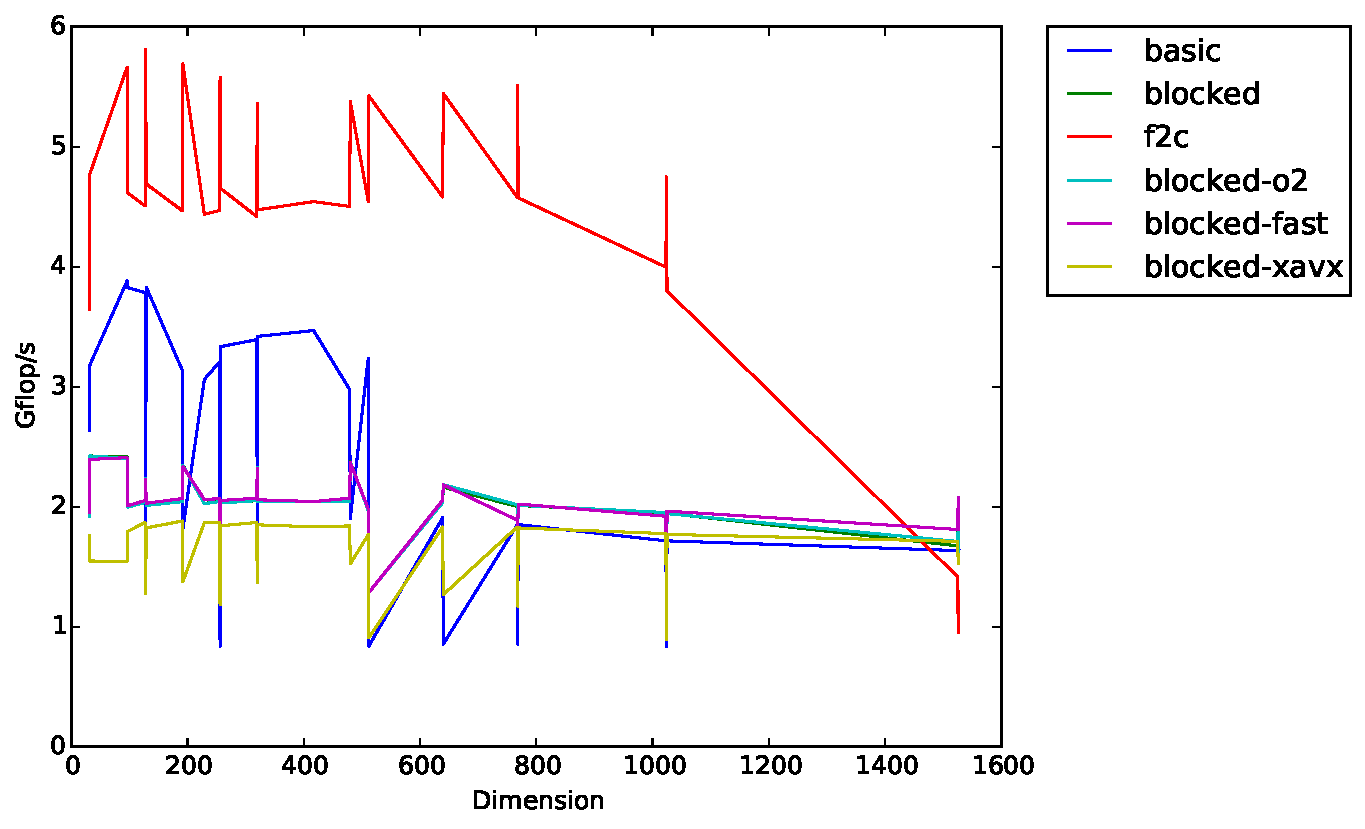
\includegraphics[width=0.7\tw]{fig-opts-comp-results.pdf}

  \caption{\textbf{Performance Comparison of Compiler Optimizations --}
    Each compiler option was applied to the naive blocked implementation
    of DGEMM. We intentionally omit the results for BLAS nad MKL
    implementations in order to focus on the behavior at the performance
    range of the optimization.}

  \label{fig-opts-comp-results}

\end{figure}


The results for using the various compiler options are shown in
Figure~\ref{fig-opts-comp-results}. Unfortunately, none of these extra
compiler options improved performance over the naive blocked
implementation. In fact, the {\tt{-xAVX}} option slightly decreased
performance. An object dump of the binary showed that the compiler was
indeed inserting vector instructions but it seems a naive
auto-vectorization can actually degrade performance. The other options
actually had roughly the same performance as the naive blocked
implementation. One interesting point to note is that the basic
implementation outperforms the blocked implementation for smaller matrix
sizes. This makes sense since the overhead of communication required
through memory between blocks is more noticeable for smaller matrices
when there is less computation per block (i.e., lower
volume-to-surface-area ratio).

\clearpage
